\documentclass[11pt]{article}
\usepackage{amsmath}
\usepackage{graphicx}
\usepackage{biblatex}
\usepackage{caption}
\graphicspath{{./images/}}
\DeclareMathOperator{\sininv}{sin^{-1}}
\newcommand{\numpy}{{\tt numpy}}    % tt font for numpy
\usepackage{url}

\topmargin -.5in
\textheight 9in
\oddsidemargin -.25in
\evensidemargin -.25in
\textwidth 7in

\begin{document}

% ========== Edit your name here
\author{Joshua Tensuan}
\title{Graphing Project}
\maketitle

\medskip

% ========== Begin answering questions here
\section{Introduction}

% ========== Just examples, please delete before submitting
Per Wikipedia, a graph is a structure amounting to a set of objects in which some pairs of the objects are in some sense "related". More specifically, these objects correspond to vertices (or nodes or points) and each of the related objects/vertices are connected by an edge. There are many types of graphs, but for this project, we focus on undirected graphs. Undirected graphs are graphs where the edges in which edges are bidirectional and do not carry a specific weight value (an edge between 2 points either exist do or do not exist). 

Graphs carry many interesting properties that are studied in the field of graph theory. In this project, we analyze a few of these properties. One property we investigate is the relationship between a certain threshold distance value and the total number of edges between points (an edge exists if 2 points are under the threshold distance) on a randomly generated $10\times 10$ Euclidean graph. Another property we investigate is the relationship between the threshold distance and probability of connectedness in a graph where again, an edge exists if 2 points are under the threshold distance, on a randomly generated $10\times 10$ Euclidean graph where connectedness is defined as when a graph has at least one vertex and there is a path between every pair of vertices. Each of these relationships are tested with varying amounts of points for both statistical replication and to analyze possible differences in the results.

In this project, we first implement a Euclidean graph class. Then, we implement methods for checking connectedness and the total number of edges given a certain threshold distance and number of points. After, we analyzed the results with differing numbers of point through multiple trials.

\section{Procedure}

Initially, we built a Euclidean graph class that utilized a point class. The point class was a simple object that stored $x$ and $y$ values on the $10 \times 10$ Euclidean graph. It also containted the basis for the random generation of these $x$ and $y$ values. The empty constructor for the point object utilized a uniform real distribution from the C standard library. The Euclidean graph class included 2 vectors: 1 vector that stored point objects that represent the vertices in a Euclidean graph and 1 vector that stored vectors of integers to represent the Euclidean graph in an adjacency matrix format. We chose to represent both of these in vectors as it facilitates size manipulation of the graph. On top of this, the Euclidean graph class contained a method to check the number of edges between points given a certain threshold distance and another method that utilized the depth first search algorithm (DFS) to check for connectedness.

We analyzed the relationship between threshold distance and total number of points across many different numbers of points. For every point, we used a certain number of trials to obtain an average number of edges. We changed this number of trials for every number of points to get an approximately equal runtime because the runtimes of the method exponentially increased with the number of points. In order to compare between different numbers of points, we divided the number of edges by the total number of edges from every point with $T = ((n \dot (n - 1)) / 2)$ where $T$ is the total number of edges, and $n$ is the number of points. This ensured that we would be able to plot a scaled down number of edges (to between 0 and 1) versus threshold distance. We then saved a text file that contained values of threshold distance and an average number of edges. Finally, we plotted this relationship on a graph, plotting multiple lines with multiple points using the command-line program gnuplot.

Again, like we did before, we analyzed the relationship between threshold distance and connectedness across many different numbers of points. Further, similar to what we did to analyze the previous relationships, we used a certain number of trials to obtain an average probability of connectedness, adjusting as needed to keep a fairly reasonable runtime. Because this value is a probability, we did not need to scale our dependent variable down to values between 0 and 1 to ease comparison between different numbers of points. Like previously, we then saved a text file that contained values of threshold distance and average probability of connectedness, plotting this relationship on a graph with multiple lines corresponding with multiple points using the command-line program gnuplot.

\section{Results}

\begin{center}
    \captionof{figure}{Graph analyzing the first relationship of threshold distance and scaled number of edges with multiple numbers of points.}
    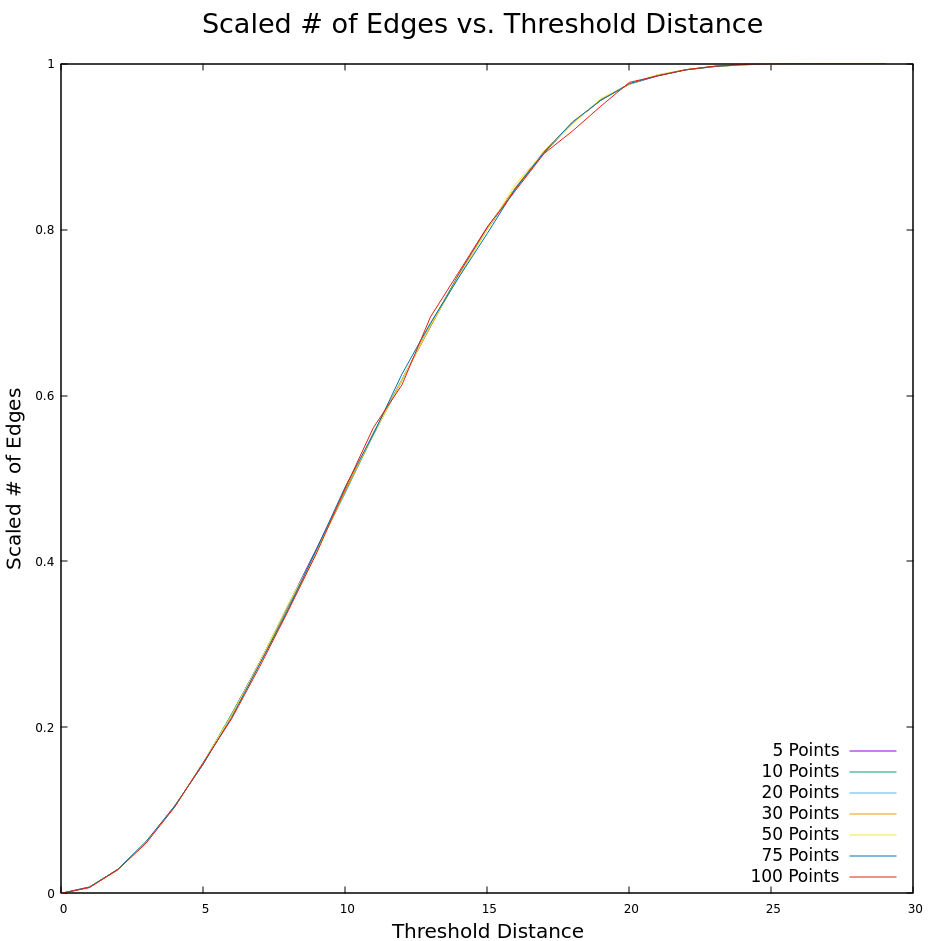
\includegraphics[scale=0.5]{Graph1.png}
\end{center}

\pagebreak

\begin{center}
    \captionof{figure}{Graph analyzing the second relationship of threshold distance and probability of connectedness with multiple numbers of points.}
    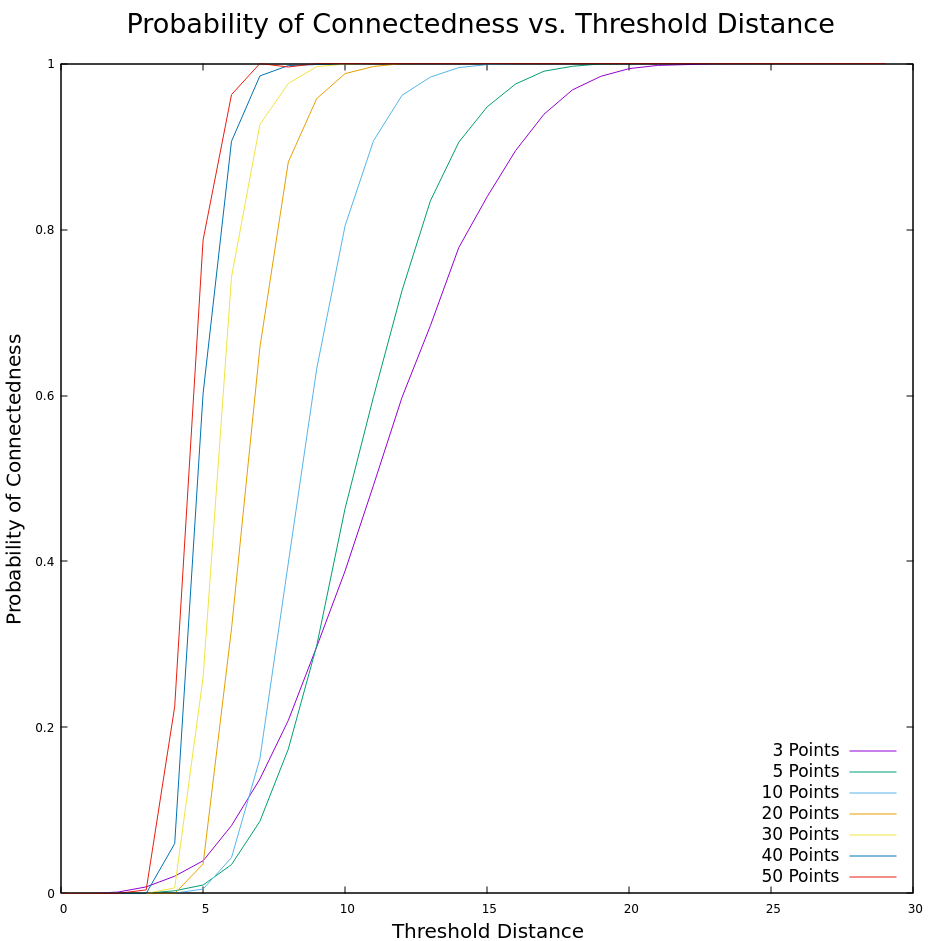
\includegraphics[scale=0.5]{Graph2.png}
\end{center}

\section{Conclusion}

Both relationships showed a sigmoidal relationship between threshold distance and the dependent variable (Number of Edges and Probability of Connectedness). Graphs of scaled number of edges versus threshold distances were effectively the same for all number of points tested. More points could not be tested due to computational limitation. Half of all possible edges occured when the threshold distance was between 11 and 12 on a Euclidean $10 \times 10$ space. In contrast, the graphs for probability of connectedness versus threshold distance were notably different. When there were more points, the probability of connectedness increased more steeply compared to when there were less points. In effect, graphs with more points would generally have a higher probability of connectedness. However, all the graphs still exhibited a common sigmoidal relationship.

Both of these results make sense intuitively. Looking at the first relationship, we know that the the scaled number of edges will start at 0 at small threshold distances then asymptotically approach the maximum number of edges as the threshold distance approaches its maximum value of 30. Looking at the second relationship, we know that the probability of connectedness will start at 0 for small threshold distances then asymptotically approach the maximum probability of 1 as the threshold distance approaches its maximum value of 30. However, the reason for why the scaled number of edges is effectively the same for graphs with varying numbers of points and the reason for why probability of connectedness is generally greater for graphs with more points is more trivial.

\end{document}
\grid
\grid